%%%% ijcai17.tex

\typeout{IJCAI-17 Instructions for Authors}

% These are the instructions for authors for IJCAI-17.
% They are the same as the ones for IJCAI-11 with superficical wording
%   changes only.

\documentclass{article}
% The file ijcai17.sty is the style file for IJCAI-17 (same as ijcai07.sty).
\usepackage{ijcai17}
% Use the postscript times font!
\usepackage{times}
\usepackage{multirow}
\usepackage{multicol}
\usepackage{array}
\usepackage{graphicx}
\usepackage[outdir=./]{epstopdf}
\usepackage{footnote}
\makesavenoteenv{table}
\usepackage{amsmath, bm}

% the following package is optional:
%\usepackage{latexsym} 

% Following comment is from ijcai97-submit.tex:
% The preparation of these files was supported by Schlumberger Palo Alto
% Research, AT\&T Bell Laboratories, and Morgan Kaufmann Publishers.
% Shirley Jowell, of Morgan Kaufmann Publishers, and Peter F.
% Patel-Schneider, of AT\&T Bell Laboratories collaborated on their
% preparation.

% These instructions can be modified and used in other conferences as long
% as credit to the authors and supporting agencies is retained, this notice
% is not changed, and further modification or reuse is not restricted.
% Neither Shirley Jowell nor Peter F. Patel-Schneider can be listed as
% contacts for providing assistance without their prior permission.

% To use for other conferences, change references to files and the
% conference appropriate and use other authors, contacts, publishers, and
% organizations.
% Also change the deadline and address for returning papers and the length and
% page charge instructions.
% Put where the files are available in the appropriate places.

\title{Learning to Extract Events without Human-annotated Text}
\author{Anonymous submission}

\begin{document}

\maketitle

\begin{abstract}
Existing event extraction systems are supervised and often learned from expert-annotated datasets, such as ACE and ERE event extraction program. However, constructing these high-quality corpora is costly, and manually annotated dataset are limited in size and coverage of event types, which makes models learned on these datasets hard to generalize. Inspired by some Freebase schemas which share similar structures with ACE event templates, we investigate the following problems in this paper: can we generate a feasible dataset for event extraction with Freebase automatically and is it possible to extract events on this dataset. We first propose four hypotheses based on our observation and produce our dataset accordingly. Then, we design a neural network model with ILP-based post inference committing to handling two challenging problems in event extraction: multi-type events and multi-word arguments. Finally, manual evaluation demonstrates that the data we generated are feasible, and experimental results of both manual and automatic evaluation prove the effectiveness of our proposed model.
\end{abstract}

\section{Introduction}
Automatically extracting events from natural text remains a challenging task in information extraction. Among diverse types of event extraction systems, the event extraction task proposed by Automatic Content Extraction (ACE) program is the most popular corpus for testing new event extraction algorithm. The ACE program defines the following terminology for event extraction:
\begin{itemize}
	\item \emph{Trigger}: the word that most clearly expresses the occurrence of an event.
	\item \emph{Argument}: a named entity that serves as a participant or attribute with a specific role in an event.
\end{itemize}

However, constructing this corpus is expensive. First, expert linguists are required to summarize a large amount of text to elaborately design templates about potential arguments for each event type. Second, rules should be explicitly stated to guide annotators. In spite of detailed annotation guidelines, there is still some disagreement between human annotators about what should (not) be regarded as triggers. For example, can a prepositional phrase trigger an event, like ``in prison'' triggers an \emph{arrest} event? Or can a portion of a word be a trigger, like ``ex'' in ``ex-husband'' trigger a \emph{divorce} event?
Besides, ACE event extraction system remains two major limitations:  first, oversimplified scenario of single-token trigger labeling and argument labeling; second, assumption that an event has only one type.

The aforementioned drawbacks of ACE event extraction system motivate us to (1) investigate the feasibility of automatic data generation, and (2) address the event extraction task in a more realistic scenario where annotated arguments are almost phrases, and some sentences express more than one events.

To achieve the first goal, we draw the inspiration from our observations on knowledge base (KB). A knowledge base stores complex structured information, and some of which shares a highly similar structure with event templates defined in ACE. Thus, any sentence that contains some participants and attributes in a particular KB entry is likely to imply an event in some way. On the other hand, recent studies \cite{mintz2009distant} have demonstrated the effectiveness of KB as distant supervision for binary relation extraction, which is another important task in information extraction. However, there is two major challenges when leveraging KB to event extraction: first, relations between an event and its arguments are more complex than binary relations. They can be represented as $\langle event\_type, argument_1, \ldots, argument_n\rangle$, which are n-ary relations with various numbers of entities. Second, there is no trigger information in any existing knowledge base. 
Therefore, we explore datasets generated based on different hypotheses about arguments to avoid the noise caused by the absence of triggers, and select the one that best fits in both quality and quantity (see Section~\ref{datagen}). Among these hypotheses, the vital one is that, for a particular event type, there are some relevant arguments, called \textbf{key arguments}, which together can trigger an event of the corresponding type and distinguish it with other event types. In this paper, we utilize Freebase as the knowledge base. And we choose Wikipedia articles as texts for data generation, according to Mintz et al. \shortcite{mintz2009distant}, because a major source of Freebase is the tabular data from Wikipedia, making it a natural fit with Freebase. Figure~\ref{fig:3} illustrates two examples of sentences annotated by our algorithm.

To achieve the second goal, unlike previous ACE event extraction systems \cite{li2013joint,chen2015event}, which regard event extraction as a classification problem, we split event extraction into two sequence labeling subtasks, namely event detection and argument detection. Following the fashion in other sequence labeling tasks, like POS tagging and NER \cite{huang2015bidirectional,lample2016neural}, we utilize a LSTM-CRF model to label key arguments and non-key arguments in the sentences separately. However, based on the above hypothesis, LSTM-CRF is not a flawless solution, as the structure of an event is not sequential and there are strong dependencies between key arguments with respect to the same event type. Therefore, we reformulate the hypotheses as constraints and apply linear integer programming on the output scores produced by LSTM-CRF to get the global optimization. After this post inference, to tackle with the multiple events and multi-type events issue, we propose a heuristic method to iteratively generate multiple labeling sequences. Finally, we conduct both manual and automatic evaluation for the detected events.

The rest of the paper is organized as follows. Section 2 presents our data generation methods, and Section 3 introduces our models of extracting events. Section 4 provides the experimental results and analyses. Section 5 discusses related work. Section 6 concludes this paper.

\section{Dataset}
\begin{figure}[h]
	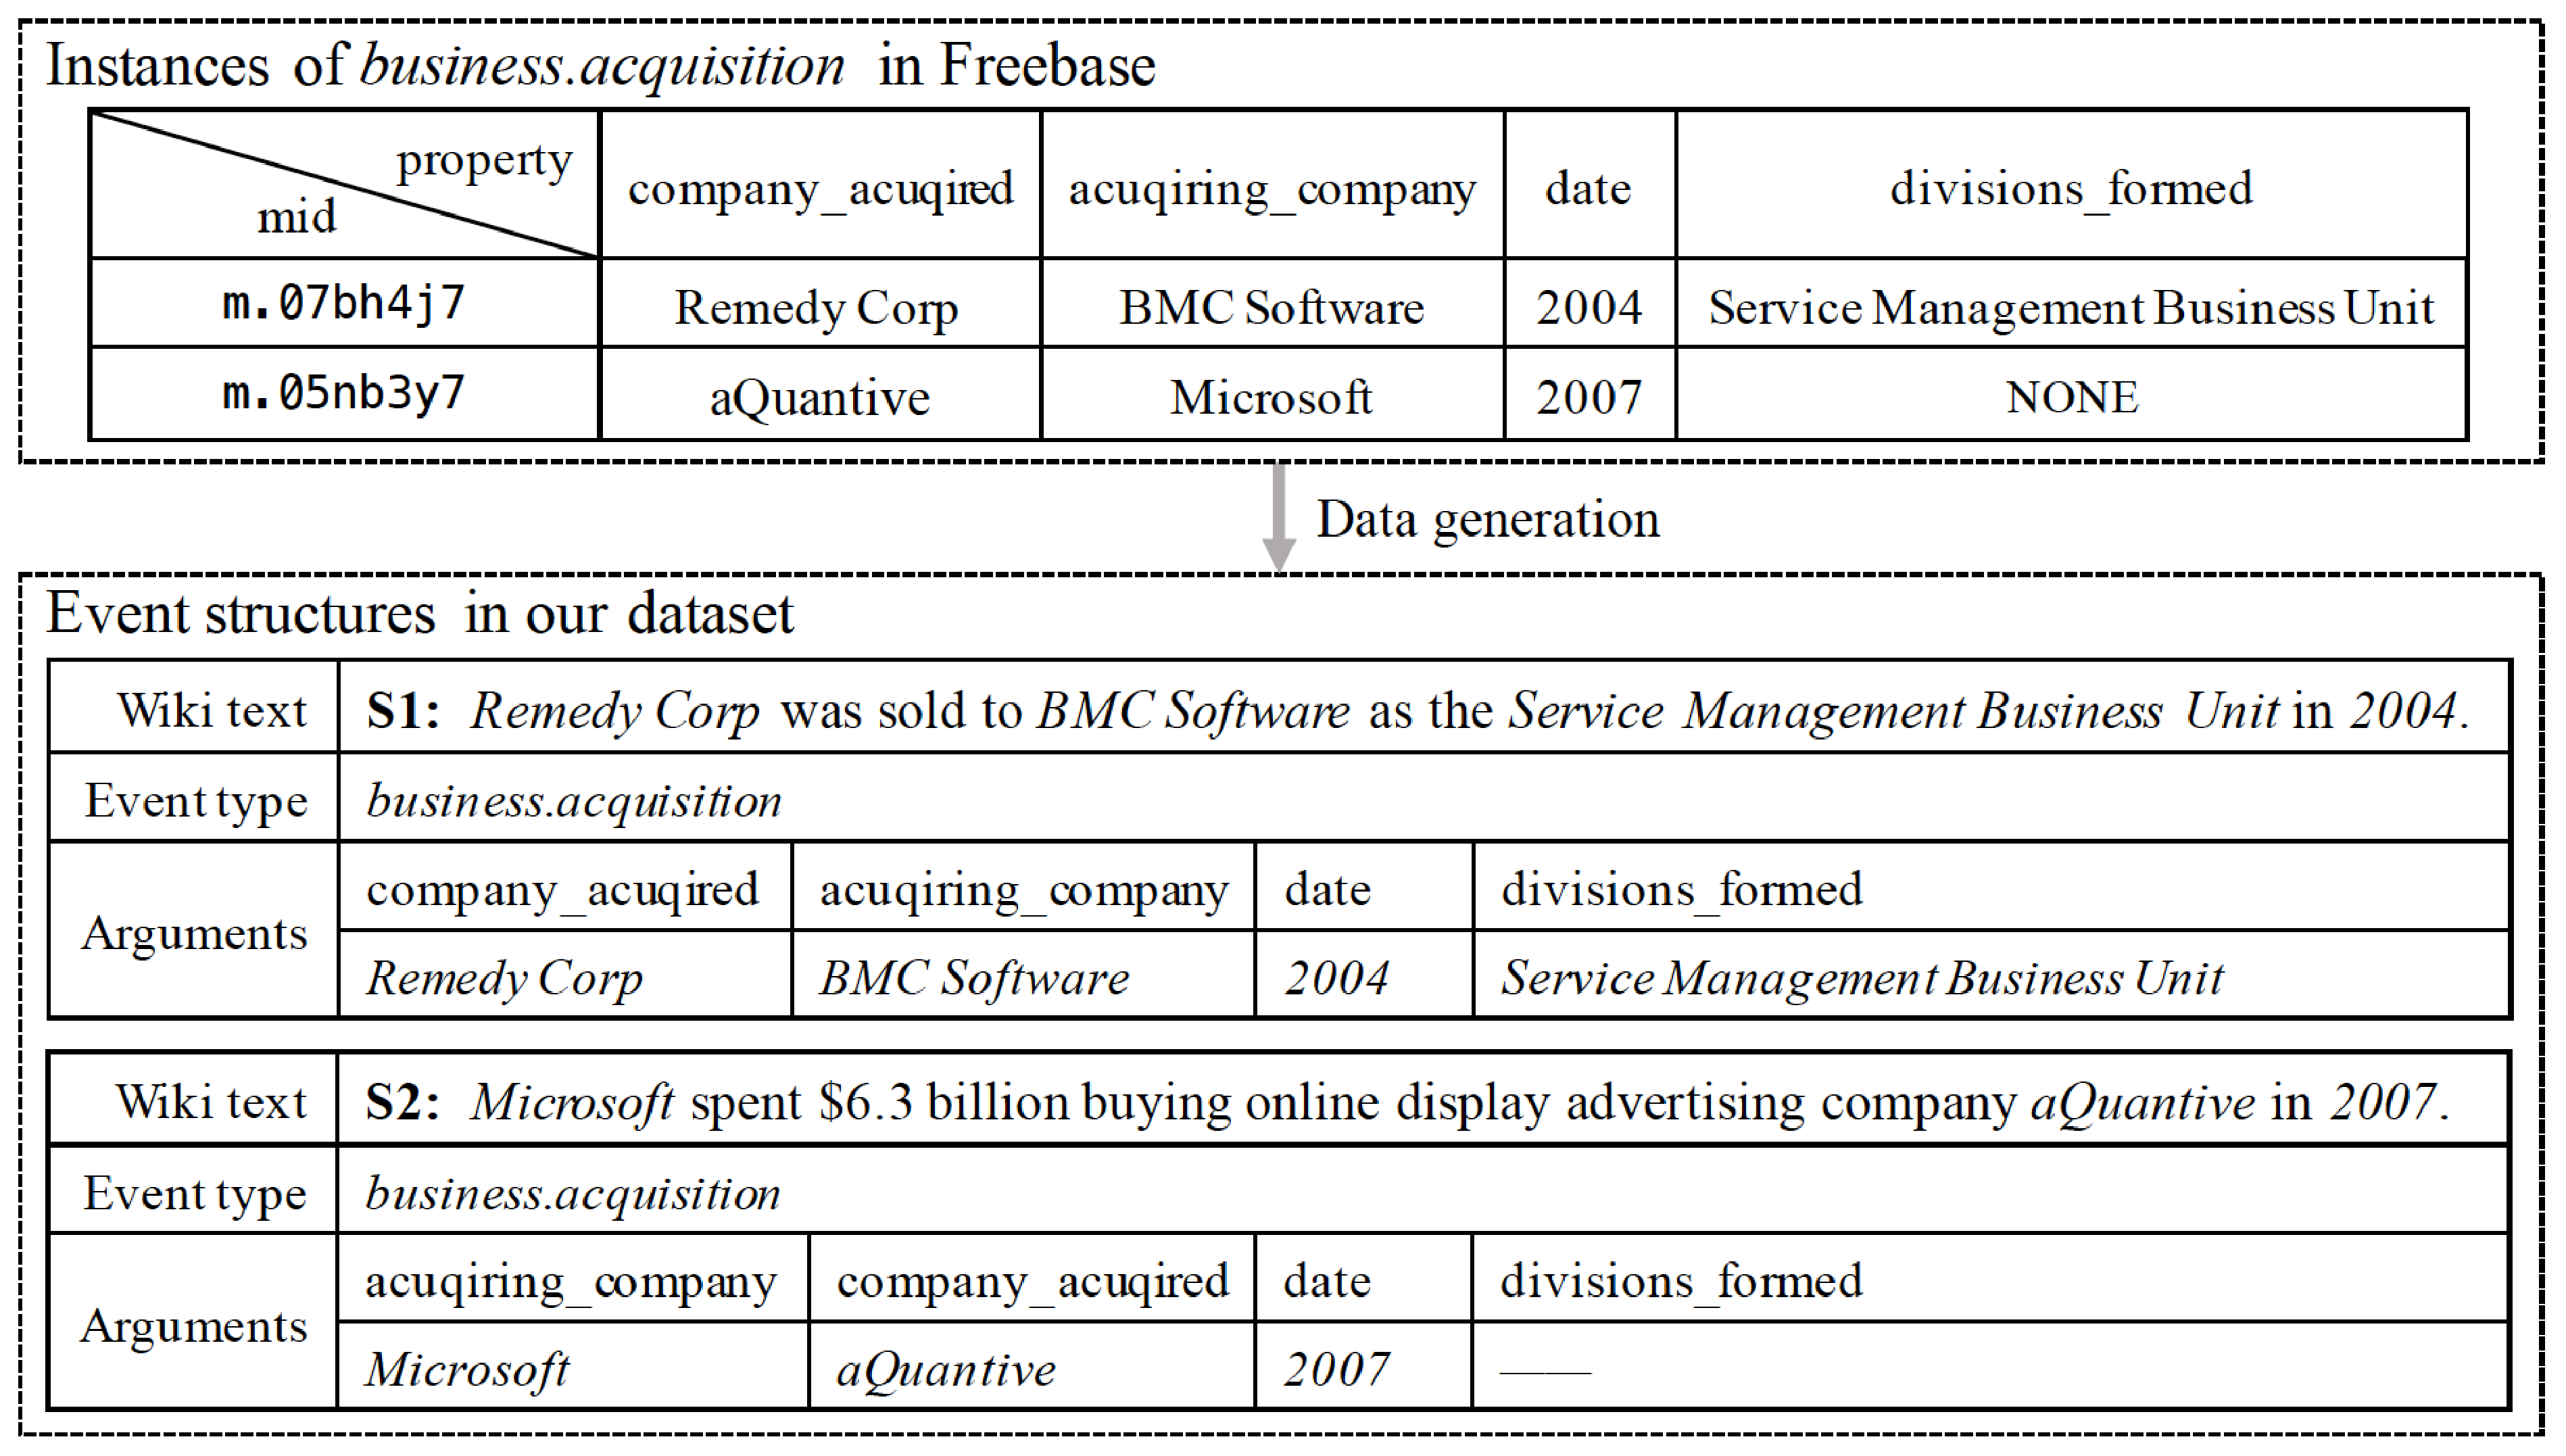
\includegraphics[width=.5\textwidth]{temp}
	\caption{Examples of CVT instances in Freebase, and labeled sentences in our dataset. \emph{Company\_acuqired}, \emph{acquiring\_company} and \emph{date} are key arguments in \emph{business.acquisition}. \label{fig:3}}
\end{figure}

\subsection{Freebase}
Freebase\cite{bollacker2008freebase} is a collaborative knowledge base where data is harvested from existing structured sources like individual, user-submitted wiki contributions.

Freebase can be divided into three layers: \emph{domain}, \emph{type} and \emph{instance}. \emph{Instances} are entries in Freebase, and are related to real-world entities like people, places and things. \emph{Types} are are different perspectives of \emph{instances}. 
%For example, the instance about \emph{Leonardo da Vinci} is assigned to three types, \emph{inventor}, \emph{painter} and \emph{scientist}. 
\textbf{\emph{Compound Value Type}} (CVT) is a special type in Freebase to represent complex data where each instance consists of multiple \textbf{\emph{properties}}. For example, in Figure~\ref{fig:3}, \emph{business.acquisition} is a CVT whose properties are \emph{company\_acquired}, \emph{acquiring\_company}, \emph{Date} and \emph{divisions\_formed}. 

We use the Freebase version of Berant et al. \shortcite{berant2013semantic}, containing 1010 CVTs. After filtering out CVTs that describe the structures of the Freebase or are irrelevant to event extraction (e.g., \emph{food.recipe\_ingredient}), we select 24 types of CVTs with around 280 million instances.

\subsection{Data Generation\label{datagen}}
We employ Freebase CVT instances to automatically annotate texts in Wikipedia. We regard a sentence as a positive one when it suggests an occurrence of event, or otherwise a negative sentence. The annotation strategy is based on four hypotheses, and we use the following examples to explain and motivate each hypothesis. S1 and S2 are positive sentences and their arguments are in italics and underlined.

\begin{quote}
	\textbf{S1}: \underline{\emph{Remedy Corp}} was sold to \underline{\emph{BMC Software}} as the \underline{\emph{Service Management Business}} Unit in \underline{\emph{2004}}.
\end{quote}
\begin{quote}
	\textbf{S2}: \underline{\emph{Microsoft}} spent \$6.3 billion buying online display advertising company \underline{\emph{aQuantive}} in \underline{\emph{2007}}.
\end{quote}
\begin{quote}
	\textbf{S3}: Microsoft hopes aQuantive’s Brian McAndrews can outfox Google.
\end{quote}
\begin{quote}
	\textbf{S4}: On April 29th, Elizabeth II and Prince Philip witnessed the marriage of Prince William.
\end{quote}

\subsubsection{H1: Positive sentences should contain all properties}
This hypothesis indicates that if a sentence has all properties of a CVT, it is more likely to be a positive sentence. We regard the CVT as event type and extract words and phrases that match the properties of a CVT instance as involved arguments. 

For example, S1 in Figure~\ref{fig:3} contains all properties of instance $m.07bh4j7$ whose type is \emph{business.acquisition}, thus we consider S1 as a positive sentence which implies an event about \emph{business.acquisition}, and \emph{BMC Software}, \emph{Remedy Corp}, \emph{Service Management Business Unit} and \emph{2004} should be labeled as the argument that plays the role of \emph{acquiring\_company}, \emph{company\_acquired}, \emph{divisions\_formed}, \emph{date}, respectively.

However, in practice, we realize that \emph{H1} is too strict that excludes a great many positive sentences like S2 in Figure~\ref{fig:3}. So we put forward the second hypothesis.

\subsubsection{H2: Positive sentences should contain all key properties}
This hypothesis is an extension of \emph{H1}, which relaxes "all properties" constraint to "key properties". We define the CVT property that has strong relevance with the occurrence of an event as \textbf{key property}. And \textbf{key argument} is the word or phrase that matches a key property of that CVT instance. 

For example, \emph{company\_acquired} and \emph{acquiring\_company} are the key properties of CVT \emph{business.accquisition}, with this relaxation, positive sentences like S2 need not contain all properties, but only key properties instead.

The relevance degree between a CVT $cvt$ and one of its property $pro$ can be measured as follows:
\begin{equation}
	score_{cvt, pro} = log \frac{count(cvt, pro)}{count(cvt) \times count(pro)} 
\end{equation}
Formula 1 simplifies the calculation of pointwise mutual information, where $count(cvt)$ is the number of all $cvt$ instances, $count(pro)$ is the number of $pro$, and $count(cvt, pro)$ is the number of $cvt$ instances that contain $pro$.

\subsubsection{H3: Key properties should include time property}
This hypothesis strengthens \emph{H2} by counting time property in key properties. We discover that for many CVTs, their key properties do not take into account time property. However, in fact, ignoring time property will produce a large number of negative sentences like S3. 

This sentence does not express an explicit event about \emph{business.accquisition} while contain all key properties of an instance, resulting in mistaking \emph{Microsoft} for \emph{acquiring\_company}, and \emph{Nokia} for \emph{company\_acquired}. By adding \emph{date} to the set of key properties, S3 will be filtered. Therefore, in \emph{H3}, we choose the property which achieves highest relevance degree among all time properties as a supplementary key property. 

\subsubsection{H4: Positive sentences should contain key properties with close syntactic distance}
We introduce another factor, syntactic distance, to annotate positive sentences. Intuitively, two arguments take participant in the same event are likely to be close in syntactic structures. This factor is feasible to eliminate negative sentences, such as S4, which satisfies \emph{H2}. 

The syntactic distance can be measured by the distance of two words in dependency parsing tree. We set the maximum distance between two key arguments as 2, denoting that, for a candidate sentence, if a pair of key arguments within it violates this constraint, it is supposed to be negative. Given the dependency parsing tree in  Figure~\ref{fig:2}, S4 is negative because the distance between \emph{Prince Philip} and \emph{marriage} is 3.

\begin{figure}
	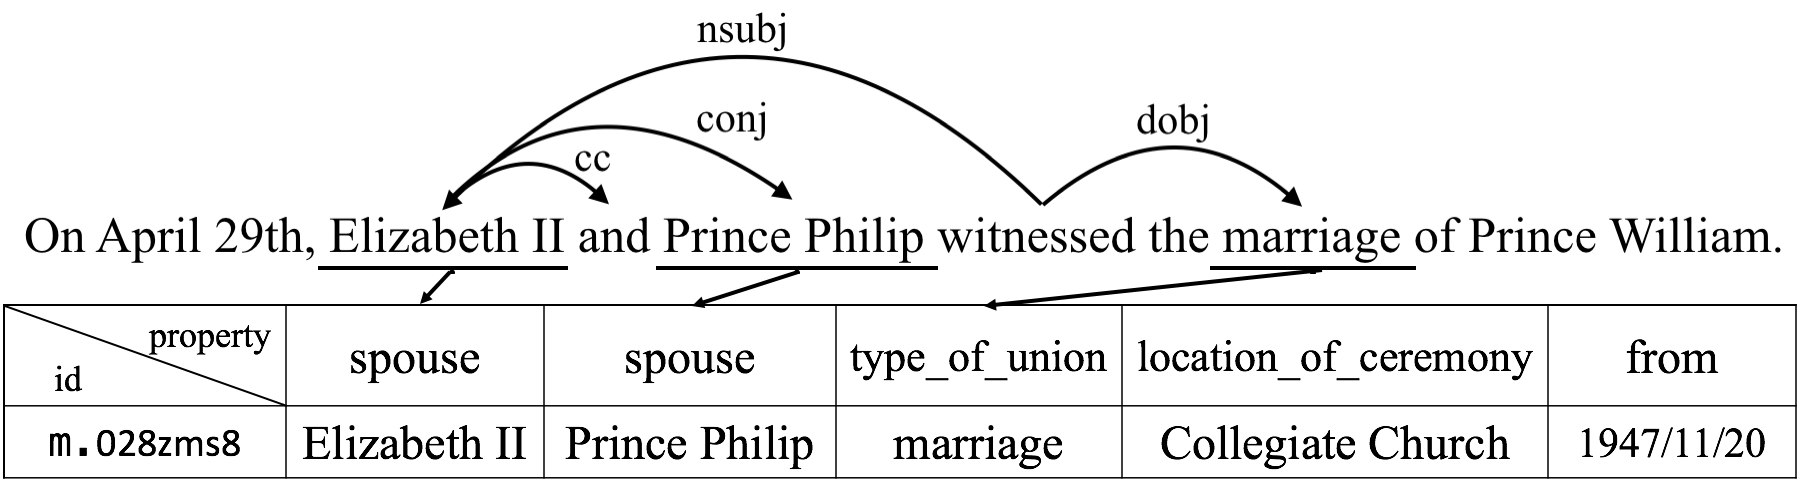
\includegraphics[width=.48\textwidth]{deppath}
	\caption{An illustration of dependency parse tree of S4. \label{fig:2}}
\end{figure}
We conduct a manual evaluation on the quantity and quality of  datasets generated by different hypotheses (see Section~\ref{sec:evalhypo}), and utilize the combinations of hypothesis \emph{H3} and \emph{H4} as the final strategy to data generation.

\section{Model}
Unlike existing event extraction work in which trigger is the key evidence to identify event and classify different event types, in the absence of human-labeled triggers, we argue that \textbf{key arguments} can play the same role as triggers. Consequently, we can treat event extraction as a pipeline of two primary subtasks, namely event detection and argument detection.
\begin{itemize}
	\item \textbf{Event detection}: to identify key arguments in the sentence. And if a sentence contains \textbf{all} key arguments of a specific event type, it is considered to imply an event of the corresponding type. For example, in S1, \emph{Remedy Corp}, \emph{BMC Software}, and \emph{2004} should be identified as \emph{business.acquisition.company\_acquired}, \emph{business.acquisition.acquiring\_company}, and \emph{business.acquisition.date} respectively. As a result, S1 should be labeled as expressing an event about \emph{business.acquisition}.
	\item \textbf{Argument detection}: to identify other non-key arguments for each event in the sentence. For the \emph{business.acquisition} event in S1, \emph{Service Management Business Unit} should be identified as \emph{business.acquisition.divisions\_formed}.
\end{itemize}

\subsection{Event Detection \label{evede}}
Before presenting our model, we need to come up with the solution to multi-words arguments. Then we introduce the components in our LSTM-CRF-ILP$_{multi}$ model one-by-one from bottom to top.

\subsubsection{Tagging scheme}
68 percent of arguments in our dataset consist of more than one words. To address this issue, we model each subtask as a sequence labeling task rather than a word classification task. Each word in the given sentence is tagged in the \texttt{BIO} scheme, where each token is labeled as \texttt{B-role} if it is the beginning of an event argument with its corresponding role \texttt{role}, or \texttt{I-role} if it is inside an argument, or \texttt{O} otherwise. 

\subsubsection{LSTM}
Long Short-Term Memory Network (LSTM) \cite{hochreiter1997long} is a natural model for sequence labeling task, which maintains a memory based on historical contextual information. Formally, given a sentence $\bm{w} = \{w_1, w_2, \dots, w_n\}$ of length $n$, we use $\textbf{x}_t$ to represent feature vector (e.g. word embedding) corresponding to the $t$-th word $w_t$. At each time step $t$, a LSTM unit takes $\textbf{x}_t$ as input and computes the output vector $\textbf{h}_t$ through several multiplicative gates. Then output vector is fed into a softmax layer to estimate a probability distribution over all possible labels.

\subsubsection{CRF}
A straightforward way is to choose the label which obtains maximum probability by LSTM as the prediction for each word. However, this independent labeling strategy is limited especially when there are strong dependencies and constraints between arguments.
% For instance, \texttt{B-acquiring\_company} is more likely to be followed by \texttt{B-company\_acquired}, while \texttt{I-company\_acquired} is not allowed to follow \texttt{B-acquiring\_company}. 
To model the correlations between labels, we introduce a CRF layer into the output of LSTM, which is widely used and proved to be effective in various sequence labeling tasks in NLP, such as POS tagging and NER \cite{collobert2011natural,huang2015bidirectional,lample2016neural}.

We consider $\textbf{P}$ to be a matrix of confidence scores output by LSTM network, and the element $\textbf{P}_{i,j}$ of the matrix denotes the probability of the label $j$ for the $i$-th word in a sentence. The CRF layer has a transition score matrix $\textbf{A}$ as parameter, where $\textbf{A}_{i,j}$ represents the score of a transition from label $i$ to label $j$. The score of a sentence $\bm{w}$ along with a path of labels $\bm{y} = \{y_1, y_2, \ldots, y_n\}$ is measured by the sum of neural network outputs and transition scores: 
\begin{equation}
	score(\bm{w}, \bm{y}) = \sum\limits_{i=0}^n\textbf{P}_{i, y_i} + \sum\limits_{i=1}^n\textbf{A}_{y_i, y_{i+1}},
\end{equation}
During test, given a sentence $\bm{w}$, we adopt the Viterbi algorithm \cite{rabiner1989tutorial} to find the optimal label sequence with the maximum score among all possible label sequences.

\subsubsection{ILP-based Post Inference}
Event detection is a structure prediction problem, while the output sequences of LSTM-CRF not necessarily satisfy the structural constraints. In other words, regardless of how many key arguments are identified correctly by LSTM-CRF, if there is one key argument missing, detection of its corresponding event is failed. To amend this flaw, we apply Integer Linear Programming (ILP) with respect to the scores given by the above LSTM-CRF model to generate the final labeling sequence.

Formally, let $\mathcal{L}$ be the set of possible argument labels. For each word $w_i$ in the sentence $\bm{w}$ and a pair of labels $ \langle l, l' \rangle \in \mathcal{L} \times \mathcal{L}$, we create a binary variable ${v_{i,l,l'} \in \{0, 1\}}$, denoting whether or not the $i$-th word $w_i$ is tagged as label $l$ and its following word $w_{i+1}$ is tagged as label $l'$ at the same time. The objective of ILP is to maximize the overall score of the variables,
\begin{displaymath}
	\sum\nolimits_{i, l, l'}v_{i,l,l'} * (\textbf{P}_{i,l}+\textbf{A}_{l,l'}) .
\end{displaymath}

We consider the following four constraints:

\textbf{C1}: Each word should be and only be labeled with one label, i.e.:
\begin{equation}
	\sum\nolimits_{l,l'}v_{i,l,l'}=1
\end{equation}

\textbf{C2}: If the value of $v_{i,l,l'}$ is $1$, then there has to be a label $l^*$ which makes $v_{i+1,l',l^*}$ equal to $1$, i.e.:
\begin{equation}
	v_{i,l,l'} = \sum\nolimits_{l^*}v_{i+1,l',l^*}
\end{equation}

\textbf{C3}: If current label is \texttt{I-arg}, then its previous label must be \texttt{B-arg}, i.e.:
\begin{equation}
	v_{i,\texttt{I-arg},l'} = v_{i-1,\texttt{B-arg},\texttt{I-arg}}
\end{equation}

\textbf{C4}: For a specific event type, its key arguments should be co-occurred, or none of them should appear in the resulting sequence. For any pair of key arguments $arg_1$ and $arg_2$ belonging to the same event type, the variables related to them are subject to:
\begin{equation}
	\sum\nolimits_{i,l'}{v_{i,\texttt{B-arg}_1,l'}} \leq n * \sum\nolimits_{j,l^*}{v_{j,\texttt{B-arg}_2,l^*}}
\end{equation}
where $n$ is the length of the sentence.

In order to address the multi-type event issue, we design a heuristic approach that iteratively produces new label sequences based on the following constraint \textbf{C5}.

\textbf{C5}: We eliminate all resulting sequences solved by ILP in the past iterations from the solution space, to obtain the next optimal sequences, i.e., for a specific sequence produced at iteration $t$, $\bm{s}^t=\{l_1^t, l_2^t, \ldots, l_n^t\}$,  
\begin{equation}
	\forall i \in {[0, n)}, v_{i,l_i^t ,l_{i+1}^t} = 0	
\end{equation}

We repeat the above procedure with these constraints through ILP, until the difference between objective value of $\bm{s}^1$ and $\bm{s}^T$ is greater than a threshold $\lambda$. Finally, we consider all sequences $\{\bm{s}^1, \bm{s}^2, \ldots, \bm{s}^{T-1}\}$ as the optimized set of label sequences. In our experiment, Gurobi \cite{gurobi} is chosen as our ILP problem solver and $\lambda=0.05 \times n$.

\subsection{Argument Detection}
After event detection, a sentence will be classified into different event types, and labeled with its corresponding key arguments. Next step is argument detection which aims to identify the remaining arguments (non-key arguments) in the sentences.  

We simply adapt the input embeddings of the LSTM-CRF model (see Section~\ref{evede}) for argument detection. Given an input sentence and one of its label sequence produced from upstream event detection task, we encode the label of each word into a key-argument feature vector through a look-up table. Then, we concatenate the word vector and key-argument feature vector as the input vector to LSTM.

\section{Experiments}

\subsection{Experimental Setup}
\subsubsection{Dataset and Evaluation Methodology}
We use the November 20th, 2016 English Wikipedia dump, and generate 7180 sentences, containing 7376 events and 25840 arguments as corpus. We then randomly select 6000 sentences for training and 1180 sentences as test set, and the remained 1200 sentences for validation. However, it costs too much time and labor annotating all sentences in the corpus, so we conducted both automatic evaluation and manual evaluation in the experiments. Specifically, we first manually evaluate the reliability of our test set. Next, we regard the noisy rule-generated data as gold standard and evaluate our model automatically. Finally, we manually evaluate a subset of events detected by our model and analysis the difference with results in automatic evaluation.

\subsubsection{Evaluation Measures}
We evaluated our models in terms of precision (P), recall (R), and F-measure (F) for each subtask. These performance metrics are computed according to the following standards of correctness:

\begin{itemize}
	\item For event type classification, an event is correctly classified if its reference sentence contains all key arguments of this event type.
	\item For argument detection, an argument is correctly detected if its offsets, role, and related event type exactly match any reference argument within the same sentence.
	\item For event detection, an event is correctly detected if its type and all its key arguments match a reference event within the same sentence.
\end{itemize}

\subsubsection{Training}
In our experiments, all hyperparameters are tuned by grid search on the development set. In different stages of event extraction, we adopted different parameters. In event detection, we set the size of word embedding to 200, the size of LSTM layer to 100. In argument detection, we use the same size of word embedding, while the size of LSTM layer is 150, and the size of key argument embedding is 50.
During training, we apply the generic stochastic gradient descent \cite{bottou2010large} with a dropout rate as 0.5 on both the input and output layers to mitigate overfitting. Word embeddings are pretrained using skip-gram word2vec model \cite{mikolov2013distributed} over the whole Wikipedia dump and fine tuned during training. 

\subsection{Generated Dataset Evaluation}\label{sec:evalhypo}
For comparison, we evaluate four dataset that utilize different hypotheses to generate positive sentences from Wikipedia. We randomly select 100 sentences in each dataset, and annotators are asked to determine whether these sentences imply events intuitively. 

\begin{table}[h]
\centering
\begin{tabular}{|l|c|c|c|c|c|} \hline
	Hypothesis & H1 & H2 & H2+H4 & H3 & H3+H4 \\ \hline
	Instances & 0.3M & 3.6M & 3.6M & 1.3M & 1.3M \\ \hline
	Dataset & 203 & 108K & 12K & 9241 & 7180 \\ \hline
	Event type & 9 & 24 & 24 & 24 & 24 \\ \hline
	Correct (\%) & 98 & 22 & 37 & 81 & 89 \\ \hline
\end{tabular}
\caption{Statistic of generated dataset with different hypotheses. Instances and Dataset denotes the number of instances and sentences that satisfy each hypothesis, respectively. Event type indicates the number of different CVT types in each dataset. Correct represents the percentage of sentences which account as stating events explicitly. \label{tab:3}}
\end{table}

As shown in Table~\ref{tab:3}, as the strictest hypothesis, \emph{H1} guarantees the quality and confidence of generated data, while there are merely 30K CVT instances that contains all properties of their corresponding CVT types. And by utilizing these instances, we can only obtain 203 sentences which cover 9 types of events, which is quite insufficient for further training. \emph{H2} is looser than \emph{H1}, though it expands the resulting dataset, it produce a large number of incorrect sentences. This side effect  demonstrates that \emph{H2} is inappropriate to be used as a soft constraint. Compared with \emph{H2}, the significant improvement in the quality of sentences generated by \emph{H3} proves that CVT properties referring time information are critical to data generation. Among all hypotheses, finally, data obtained by a combination of \emph{H3} and \emph{H4} achieves highest precision, which demonstrates that our hypothesis \emph{H3} and \emph{H4} are feasible and it is an effective way to generate reliable data automatically.

\subsection{Baselines}
To investigate the effectiveness of our proposed model, we develop three baseline extraction systems for comparison, including traditional feature-based methods and neural network models. 

For neural network method, we train a long short-term memory network that takes word embeddings as the input, and simply learns a probability distribution over all possible labels.

For feature-based methods, we apply Conditional Random Field \cite{lafferty2001conditional} and Maximum Entropy \cite{berger1996maximum} to explore a variety of elaborate features which are widely used in traditional ACE event extraction. And both two classifiers share the same feature sets.

\subsubsection{Lexical Features}
\begin{enumerate}
	\item Unigrams and bigrams of the current word and its context within a window of size 2.
	\item Unigrams and bigrams of part-of-speech tags of the current word and its context within a window of size 2.
	\item Unigrams and bigrams of lemmas of the current word and its context within a window of size 2.
	\item Synonym set entries in WordNet \cite{miller1995wordnet} of the current token.
\end{enumerate}

\subsubsection{Syntactic Features}
\begin{enumerate}
	\item The depth of the current words in the parse tree.
	\item Dependent and governor words of the current token.
	\item The path from root to leaf node of the current word in the parse tree.
\end{enumerate}

\subsubsection{Entity Information}
\begin{enumerate}
	\item Unigrams and bigrams of named entity mention of the current word and its context words and its context within a window of size 2.
	\item Relative distance and entity type of the nearest entity to the current token in the parse tree.
	\item Relative distance and entity type of the nearest entity to the current token in the sentence.
\end{enumerate}

We derive these features using Stanford CoreNLP \cite{manning2014stanford}, and apply the implementation from the CRF++ toolkit \cite{kudo2005crf++} and Le Zhang \footnote{https://github.com/lzhang10/maxent} to train CRF and max entropy classifiers, respectively.

\subsection{Automatic Evaluations}
Table~\ref{tab:1} presents the overall performance of all methods on the full test set. 

\begin{table*}[!t]
\centering
\begin{tabular}{|l|p{0.8cm}<{\centering}|p{0.8cm}<{\centering}|p{0.8cm}<{\centering}|p{0.8cm}<{\centering}|p{0.8cm}<{\centering}|p{0.8cm}<{\centering}|p{0.8cm}<{\centering}|p{0.8cm}<{\centering}|p{0.8cm}<{\centering}|} \hline
	\multirow{2}{*}{Model} & \multicolumn{3}{c|}{Event Classification} & \multicolumn{3}{c|}{Argument Detection} & 
	\multicolumn{3}{c|}{Event Detection} \\ \cline{2-10}
	 & P & R & F & P & R & F & P & R & F \\ \hline
	CRF & 96.8 & 9.93 & 18.0 & 64.8 & 6.54 & 11.9 & 29.8 & 3.06 & 5.55 \\ \hline
	MaxEnt & \textbf{97.9} & 11.4 & 20.3 & 64.5 & 7.28 & 13.1 & 29.3 & 3.40 & 6.08 \\ \hline
	LSTM & 97.2 & 62.4 & 75.1 & 77.1 & 53.9 & 63.5 & 51.0 & 32.8 & 39.9  \\ \hline \hline
	LSTM-CRF & 97.3 & 67.2 & 79.5 & \textbf{78.0} & 60.2 & 68.0  & \textbf{54.4} & 37.6 & 44.4  \\ \hline
	LSTM-CRF-ILP$_{1}$ & 93.4 & 81.4 & 86.9 & 74.1 & 71.1 & 72.6  & 49.6 & 43.3 & 46.2 \\ \hline
	LSTM-CRF-ILP$_{multi}$ & 93.2 & \textbf{81.9} & \textbf{87.2} &  74.0 & \textbf{71.5} & \textbf{72.7} & 49.5 & \textbf{43.5} & \textbf{46.3} \\ \hline
\end{tabular}
\caption{Overall system performance of automatic evaluations. (\%) \label{tab:1}}
\end{table*}

\subsubsection{Comparison with baselines}
Traditional feature-based models are inefficient in both event detection and argument detection. Although they can achieve high precisions in event classification and argument detection, they can only extract a limited number of events, resulting in low recalls. Neural-network-based methods performs much better than feature-based models, because they can make better use of word semantic features, especially, LSTM can capture longer range dependencies and richer contextual information instead of neighborly word features. Moreover, neural-network-based methods can avoid errors propagating from other NLP preprocessing tools like POS tagging and NER.

\subsubsection{Effect of CRF Layer}
Every model which has a CRF layer over its neural network output layer is superior to the one with a simple LSTM layer. Compared with LSTM model, LSTM-CRF achieves higher precisions and recalls in all subtasks by significantly reducing the invalid labeling sequences (e.g., \texttt{I-arg} appears right after \texttt{O}). During prediction, instead of tagging each token independently, LSTM-CRF takes into account the constraints between neighbor labels, and increases the cooccurrences of key arguments with regard to the same event type in some way.

\subsubsection{Effect of Post Inference}
As shown in Table~\ref{tab:1}, post inference based on ILP considerably improve the overall system performance, especially in event classification. With the help of constraint \textbf{C4},  some dubious key arguments can be inferred through other key arguments from their contexts. Compared with LSTM-CRF, LSTM-CRF-ILP$_1$ produces a gain of 7.4 in event classification, 1.8 in event detection, and 4.6 in argument detection, with respect to the F1 score.

We further investigate the effect of our heuristic method, LSTM-CRF-ILP$_{multi}$ which deals with the multi-event sentence issue. Compared with other models, LSTM-CRF-ILP$_{multi}$ selects several labeling sequences according to their objective value, and extract a number of events with comparable confidences from a sentence. As we can see from Table~\ref{tab:1}, this strategy may detect multiple events for a sentence, contributing to the increase of recalls, and F1 scores at the spent of a little drop of precisions. 

\subsection{Manual Evaluations}
\subsubsection{Manual Annotations}
We randomly sample 150 unlabeled sentences from test data set. Annotators are asked to fully annotate the events and arguments to each sentence following steps below: 

\begin{enumerate}
	\item First, determine whether a given sentence is positive or negative, in other words, whether there are events in the sentence or not.
	\item Second, assign event types to the positive sentences identified in first step.
	\item Finally, label all related arguments and their roles according to the types of events in the positive sentences.
\end{enumerate}

To make the annotation more credible, each sentence is independently annotated by two annotators, and the inter-annotator agreement is \% for event types and \% for arguments.

\subsubsection{Results}
Table~\ref{tab:2} presents the average results of manual evaluations where we measure precision, recall and F1 by the same standards of correctness as automatic evaluation.  

\begin{table*}[t]
\centering
\begin{tabular}{|l|p{0.8cm}<{\centering}|p{0.8cm}<{\centering}|p{0.8cm}<{\centering}|p{0.8cm}<{\centering}|p{0.8cm}<{\centering}|p{0.8cm}<{\centering}|p{0.8cm}<{\centering}|p{0.8cm}<{\centering}|p{0.8cm}<{\centering}|} \hline
% \begin{tabular}{|l|c|c|c|c|c|c|c|c|c|} \hline
	\multirow{2}{*}{Model} & \multicolumn{3}{c|}{Event Classification} & \multicolumn{3}{c|}{Argument Detection} & 
	\multicolumn{3}{c|}{Event Detection} \\ \cline{2-10}
	 & P & R & F & P & R & F & P & R & F \\ \hline
	CRF & 88.9 & 12.0 & 21.2 & 56.7 & 7.56 & 13.3 & 22.2 & 3.0 & 5.3 \\ \hline
	MaxEnt & \textbf{92.9} & 9.78 & 17.7 & 61.7 & 6.44 & 11.7 & 28.6 & 3.01 & 5.44 \\ \hline
	LSTM & 91.3 & 71.4 & 80.2 & 70.9 & 60.2 & 65.1 & 48.1 & 37.6 & 42.2 \\ \hline \hline
	LSTM-CRF & 89.3 & 75.2 & 81.6 & \textbf{72.8} & 64.9 & 68.6 & \textbf{48.2} & 40.1 & 44.1  \\ \hline
	LSTM-CRF-ILP$_{1}$ & 85.1 & \textbf{85.7} & 85.4 & 67.6 & 72.9 & 70.2 & 44.0 & 44.4 & 44.2 \\ \hline
	LSTM-CRF-ILP$_{multi}$ & 85.6 & 86.5 & \textbf{85.5} & 67.4 & \textbf{73.6} & \textbf{70.4} & 44.1 & \textbf{45.1} & \textbf{44.6} \\ \hline
\end{tabular}
\caption{Average of overall system performance of manual evaluations. (\%) \label{tab:2}}
\end{table*}

\begin{figure}[h]
	\centering
	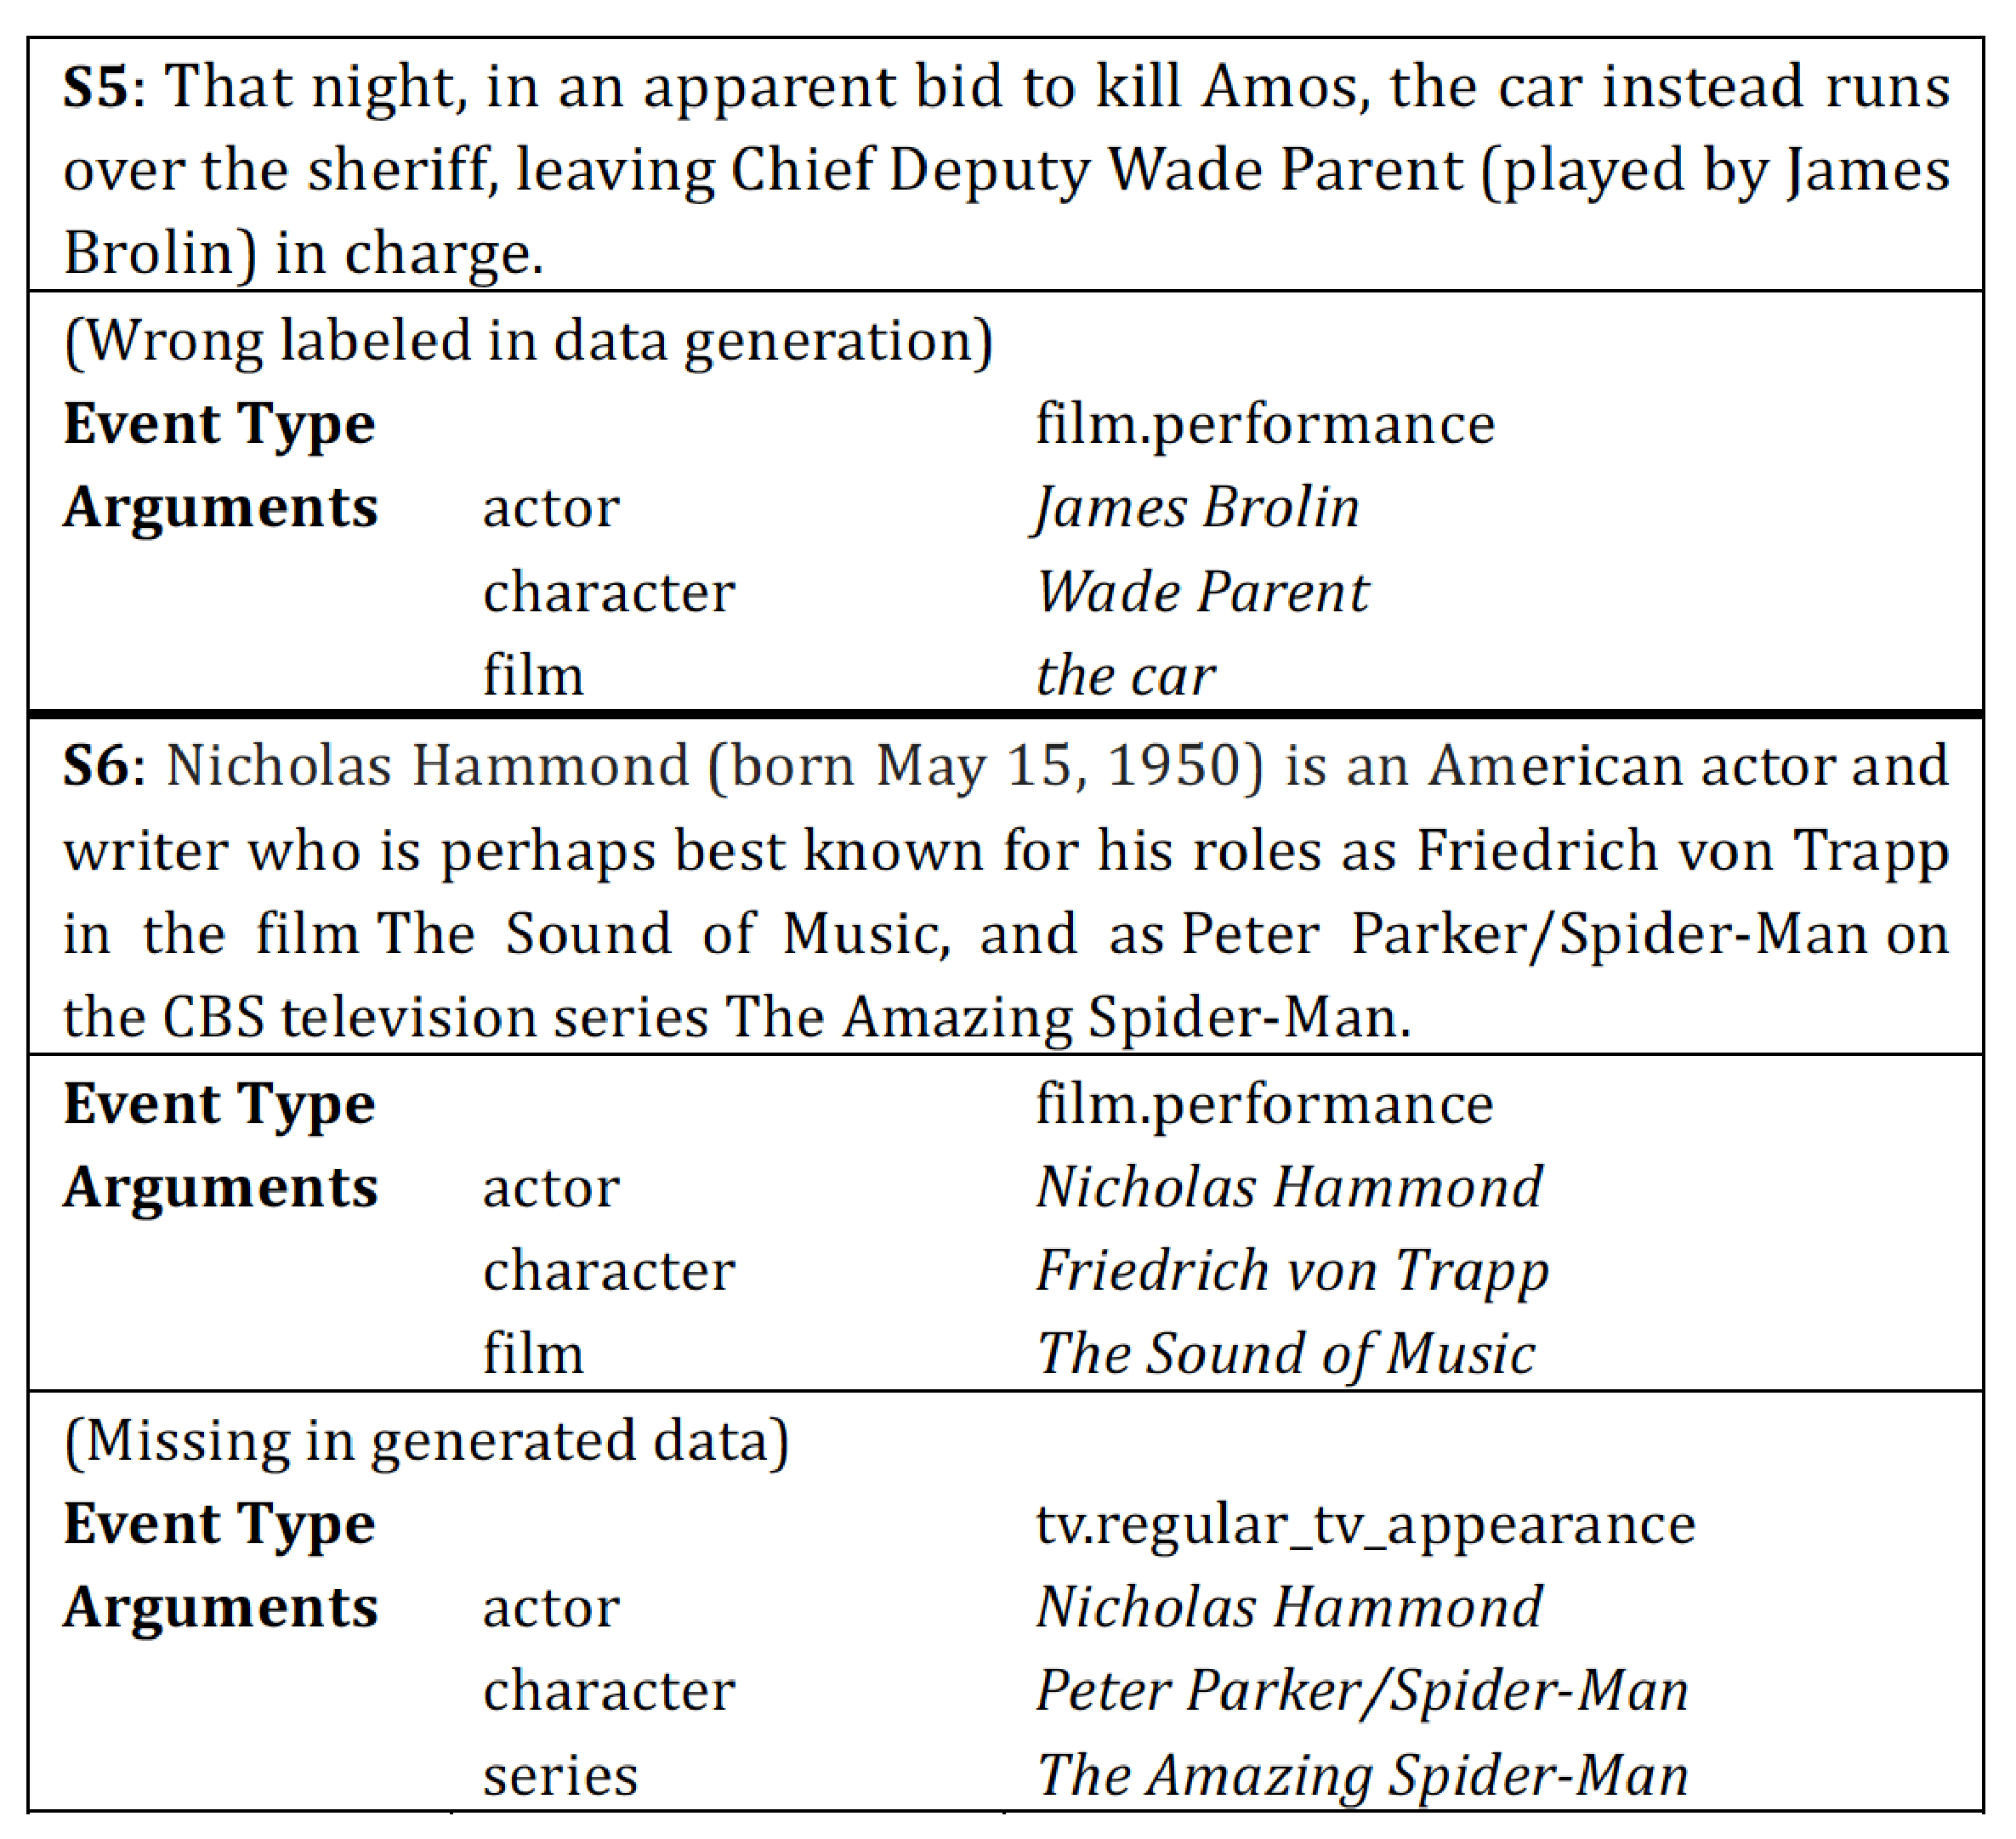
\includegraphics[width=.45\textwidth]{example.eps}
	\caption{Example outputs of LSTM-CRF-ILP$_{multi}$.\label{fig:1}}
\end{figure}

We can draw similar conclusions about the comparison of performances between different models as automatic evaluation. We demonstrate that LSTM-CRF-ILP$_{multi}$ is the most effective model in event extraction as it attains the highest F1 score in both manual and automatic evaluation.

Moreover, manual evaluation helps us to gain a deep insight of our generated data and proposed models. We further conduct automatic evaluation on this manual annotated dataset and list the top 5 event types whose F1 scores of LSTM-CRF-ILP$_{multi}$ differ greatly from automatic evaluation in Table~\ref{tab:4}. 

\begin{table}[h]
\centering
\begin{tabular}{|l|c|c|c|} \hline
	Event type & P & R & F \\ \hline
	olympics.medal\_honor \footnote{The full name is olympics.olympic\_medal\_honor in Freebase.} & $\downarrow$ 25.0\% & $\downarrow$ 5.0\% & $\downarrow$ 13.8\% \\ \hline
	film.performance & $\downarrow$ 21.4\% & $\uparrow$ 3.1\% & $\downarrow$10.3\% \\ \hline
	business.acquisition & $\rightarrow$ & $\downarrow$ 7.1\% & $\downarrow$ 5.4\% \\ \hline
	tv.appearance \footnote{The full name is tv.regular\_tv\_appearance in Freebase.} & $\downarrow$ 9.5\% & $\uparrow$ 3.0\% & $\downarrow$ 3.1\% \\ \hline
	film.release \footnote{The full name is film.film\_regional\_release\_date in Freebase.} & $\downarrow$ 7.7\% & $\uparrow$ 5.6\% & $\downarrow$ 0.55\% \\ \hline
\end{tabular}
\caption{Top 5 event types whose performances on event classification differ most from automatic evaluation. The model we evaluated is LSTM-CRF-ILP$_{multi}$ \label{tab:4}}
\end{table}

Most of the performance differences blame on the stage of data generation. Figure~\ref{fig:1} examples two types of errors in data generation. Some of the sentences automatic generated test set are noisy, in other words, they do not imply any event while still match all key properties of certain instances. Take S5 as an example, though the phrases \emph{the car} matches a film name, it does not indicate this film, and there is no explicit evidence expressing that an actor starring in a film. This is a bottleneck of our data generation strategy. During manual evaluation, we find 16 negative sentences and all of them are mistakenly labeled due to the same reason. Unfortunately, our model fails to identify some of these negative sentences.

Remarkably, our LSTM-CRF-ILP$_{multi}$ model can help find more CVT instances that not referenced in Freebase. There are two events mentioned in S6, while the arguments of the second event do not match any CVT instances in Freebase, leading to an omitting event in data generation. This phenomenon suggests that learning from distant supervision provided by Freebase, our model can help complete and update properties of Freebase instances in return.

\section{Related Work}

\section{Conclusions and Future Work}
Motivated by the data labeling problem in ACE event extraction system, we explore a method to generate training data automatically based on four hypotheses between arguments and events. The manual evaluation result demonstrates that our hypotheses are feasible, and the produced dataset is clean and high-quality.

In addition, we propose a LSTM-CRF model with a ILP-based post inference approach to perform event extraction on the auto-generated data. Experimental results of both manual and automatic evaluation show that our model can not only extract simple events, but also multi-type events and multiple events within one sentence.

Furthermore, we find that our model can extract information not collected by Freebase. In the future, we intend to explore an approach to extend this work to knowledge base population. 

% \section*{Acknowledgments}

%% The file named.bst is a bibliography style file for BibTeX 0.99c
\bibliographystyle{named}
\bibliography{ijcai17}

\end{document}

